\chapter{Overall description}
\labch{options}
	\section{Product perspective}
		\subsection{Scenarios}
			\textbf{Student signs up to S\&C}
			\begin{flushleft}
				Student Bob enters in the system for the first time. On the homepage, he first clicks the \emph{Registration button} and then the \emph{Student Registration button}. To register, Bob fills out a form providing its institutional e-mail (bob.johnson@mail.polimi.it) and password (which will be used for future logins), a brief description of his academic background and specifies whether he would like to take part to the recommendation analysis. Finally, Bob uploads his CV by clicking the \emph{Upload CV button}. Now Bob is registered and can search for internships that interest him.
			\end{flushleft}
			\textbf{Company signs up to S\&C}
			\begin{flushleft}
				The company FinestraMI enters the system for the first time. On the homepage, it first clicks the \emph{Registration button} and then the \emph{Company Registration button}. To register, the company fills out a form providing its name, a brief description of its area of expertise and its business area (the market where it operates) and finally its corporate e-mail (info@finestrami.it) and password (which will be used for future logins). FinestraMI also specifies, by selecting the appropriate option, whether it wants take part into the recommendation analysis. Now, FinestraMI is registered and can publish its internships advice.
			\end{flushleft}
			\textbf{Company publishes an internship offer}
			\begin{flushleft}
				The company FinestraMI enters in the system; on the homepage, it clicks the \emph{Login button}. Once logged in, FinestraMI accesses the \emph{Publish New Internship section}. A new internship advice is added by filling out a form where the following information is provided:
				\begin{itemize}
					\item "Window restore" (the intership title);
					\item "The aim of this internship is to give to student to opportunity to repair office windows and..." (a brief description);
					\item "third year bachelor students..." (experience required);
					\item "not suffering from dizziness" (desired skills);
					\item "1. coordination of glass disposal; 2. ..." (main activities the internship involves);
					\item "no paid, canteen tickets available" (terms of the internship);
					\item "22/11/2024" (advice deadline).
				\end{itemize}
				
				Now the internship advice is visible to students registered on the platform (and also to FinestraMI).
			\end{flushleft}
			\textbf{Student proactively searches for an internship}
			\begin{flushleft}
				Students Bob, Alice and Micheal access to the system by clicking "Login". Each one of them wants to find an internship to apply but each one of them has a different idea of what and where he/she would like to do/be:
				\begin{itemize}
					\item Bob is really interested on doing practice on an handwork but he neither knows a name of a company nor knows which kind of handwork apply for so, he goes to the \emph{View Internships section}, where he can see all the published internships, listed from the most recent to the least recent. The most recent one is "Window restore" by FinestraMI, then he selects it;
					\item Alice has not already decided the kind of internship she wants to apply for but knows many names of companies that operate near her home and so she prefers to go to the \emph{View Companies section}, where she can see all the registered companies and all the internships published by each company. Then she recognized FinestraMI and since she knows that it is expanding, she decides to select it. "Window restore" is the only available advice of FinestraMI but she select it anyways;
					\item Micheal is looking forward to do an internship related to windows restoration, so he uses the search bar to insert "windows restoration" and selects the option "only paid internships", but no internship are found. Then he removes the option and find the internship of FinestraMI. Since it is the only left, he selects it.
				\end{itemize} 
			\end{flushleft}
			\textbf{Student receive a notification about a new internship}
			\begin{flushleft}
				The company CancellaMI (previously registered to the platform) publishes a new internship related to railings maintenance then, Student Bob, who has chosen to be notified by the system when new internships that might be of interest are published, receives an email informing it that a new intership related to his studies is available, since it stated in his CV that after the internship at FinestraMI he became passionate of railings. Bob then logs into the platform and, by going to the \emph{Notification section}, can view the internships offer in more detail.
			\end{flushleft}
			\textbf{Company receives a notification about new possibly interested students}
			\begin{flushleft}
				Company FinestraMI, which has chosen to be notified by the system, receives an email informing it that new students are appealing for its intership "Window Restore" (based on their CVs). FinestraMI then logs into the platform, goes into the \emph{Internship section}, clicks on \emph{Windows restore internship} and by going to the \emph{Notification section} can view the students'profiles and their CVs in more detail.
			\end{flushleft}
			\textbf{Student applies for an internship}
			\begin{flushleft}
				Student Bob wants to apply for the internship "Windows restore". To do so, they log into the system, access the page for "Windows restore" internship and click the \emph{Apply button}. Automatically, the system will send a notification to FinestraMI (the company offering the internship) to inform it that Bob has applied
			\end{flushleft}
			\textbf{The company accepts the application of a student}
			\begin{flushleft}
				Company FinestraMI receives the email regarding student Bob's application for the internship "Window Restore". FinestraMI then logs into the platform, navigates to the \emph{Internships section}, select the \emph{Window Restore Internship}, goes to the \emph{Notification section} and clicks the \emph{Accept Application button} to approve Bob's application.
			\end{flushleft}
			\textbf{The company proposes to a student to apply for one of its internships}
			\begin{flushleft}
				The company FinestraMI consults its list of recommended students for Window Restore and send a proposal to Bob Jones (by clicking on the dedicated button). Soon after the system sends a notification of the proposal to Bob. 
			\end{flushleft}
			\textbf{Student accepts an internship proposal}
			\begin{flushleft}
				Bob receives an email regarding Window Restore proposal (of the company FinestraMI), then Bob logs into the platform, navigates to the notification section, open the notification regarding the proposal and clicks on the accept button.
			\end{flushleft}
			\textbf{The application deadline expires and the selection process is configured}
			\begin{flushleft}
				The administrator of the company FinestraMI notices that the application deadline for the internship advice "Window Restore" (which was previously published on the platform) is now expired and selection process for that internship has not configured yet, so he goes to the designated page and configures:
				\begin{itemize}
					\item two steps (the selection process will be made up of two steps);
					\item a set of metrics to evaluate students ("manual skills" and "knowledge of materials" in this case);
					\item each step is configured as a questionnaire with a series of questions for the students, in this case in particular:
						\begin{enumerate}
							\item first step is test of both open and closed questions regarding knowledge of materials. For closed questions, the platform is also able to automatically check if they are corrected or not (and so, for each closed question, also the scores to assign to each possible answer are inserted into the system). Open questions will be evaluated manually by the company;
							\item second step is an oral exam. Since there are no predefined questions for this step, the company only inserts into the system one open question called "oral exam", scores will be inserted by the company at the end of the exam.
						\end{enumerate}
					\item for each step and for each candidate, the company chooses also the date in which it provides the questionnaire to the candidate.
				\end{itemize}
			\end{flushleft}
			\textbf{The selection process runs}
			\begin{flushleft}
				For the internship advice "Window restore", the company FinestraMI received three applications: Bob, Alice and Micheal. FinestraMI is planning to accept only one student at time, therefore it chooses to first call Micheal for the first step, since his curriculum impressed more the company. On \date{23/11/2024} Micheal is called and the questionnaire is given to him. His answers are evaluated (automatically for the closed ones and manually for the opened ones) and gets an overall score of 99 out of 100: the company decides to select him, discards Bob's application and leaves suspended the call for Alice. The company sets for Bob and Micheal the right message and the platform notifies them. 
			\end{flushleft}
			\textbf{User provides a feedback at the end of the selection process}
			\begin{flushleft}
				Micheal has just received the selection results for his application for the "Window restore" internship of FinestraMI. Attached to it, the system provides him an optional questionnaire where it asks to Micheal to evaluate his experience of the selection (questions are quite standard, such as "was the company on time with the interview appointments?", "did the questions related to the required skills" e.c.c.). Since it is not compulsory, Micheal does not compile it. On the other side, once the entire selection process of FinestraMI is closed, FinestraMI receives from the system a questionnaire to evaluate its experience (questions mainly concern the preparation level of the candidates, such as "was the number of students with the required skills below average?"). Then the company compiles it from the system.
			\end{flushleft}
			\textbf{User reports a complaint on one of the internship is currently doing}
			\begin{flushleft}
				Today, Alice who is currently enrolled in the internships at the company WeWorkGreat had a problem with the task that was given to her, she asks the helpdesk of the company where she is performing the internship and they ask her to upload a video on the company file sharing platform to show the situation. Alice notices that she can’t upload the video because the maximum uploading size for students is to 10 MB, then she opens Students\&Companies and writes a compliant that states that the file sharing system of WeWorkGreat is only of 10 MB.
			\end{flushleft}
			\textbf{User provides a feedback at the conclusion of an internship}
			\begin{flushleft}
				Alice has just finished the internship at WeWorkGreat, an non-compulsory questionnaire is given to her with some general questions related to her experience at the company (e.g. "did the company respect the terms listed in the advice?" e.c.c.). Since it is not compulsory, Alice decides to not compile it.
			\end{flushleft}
		\subsection{High-level class diagram}
			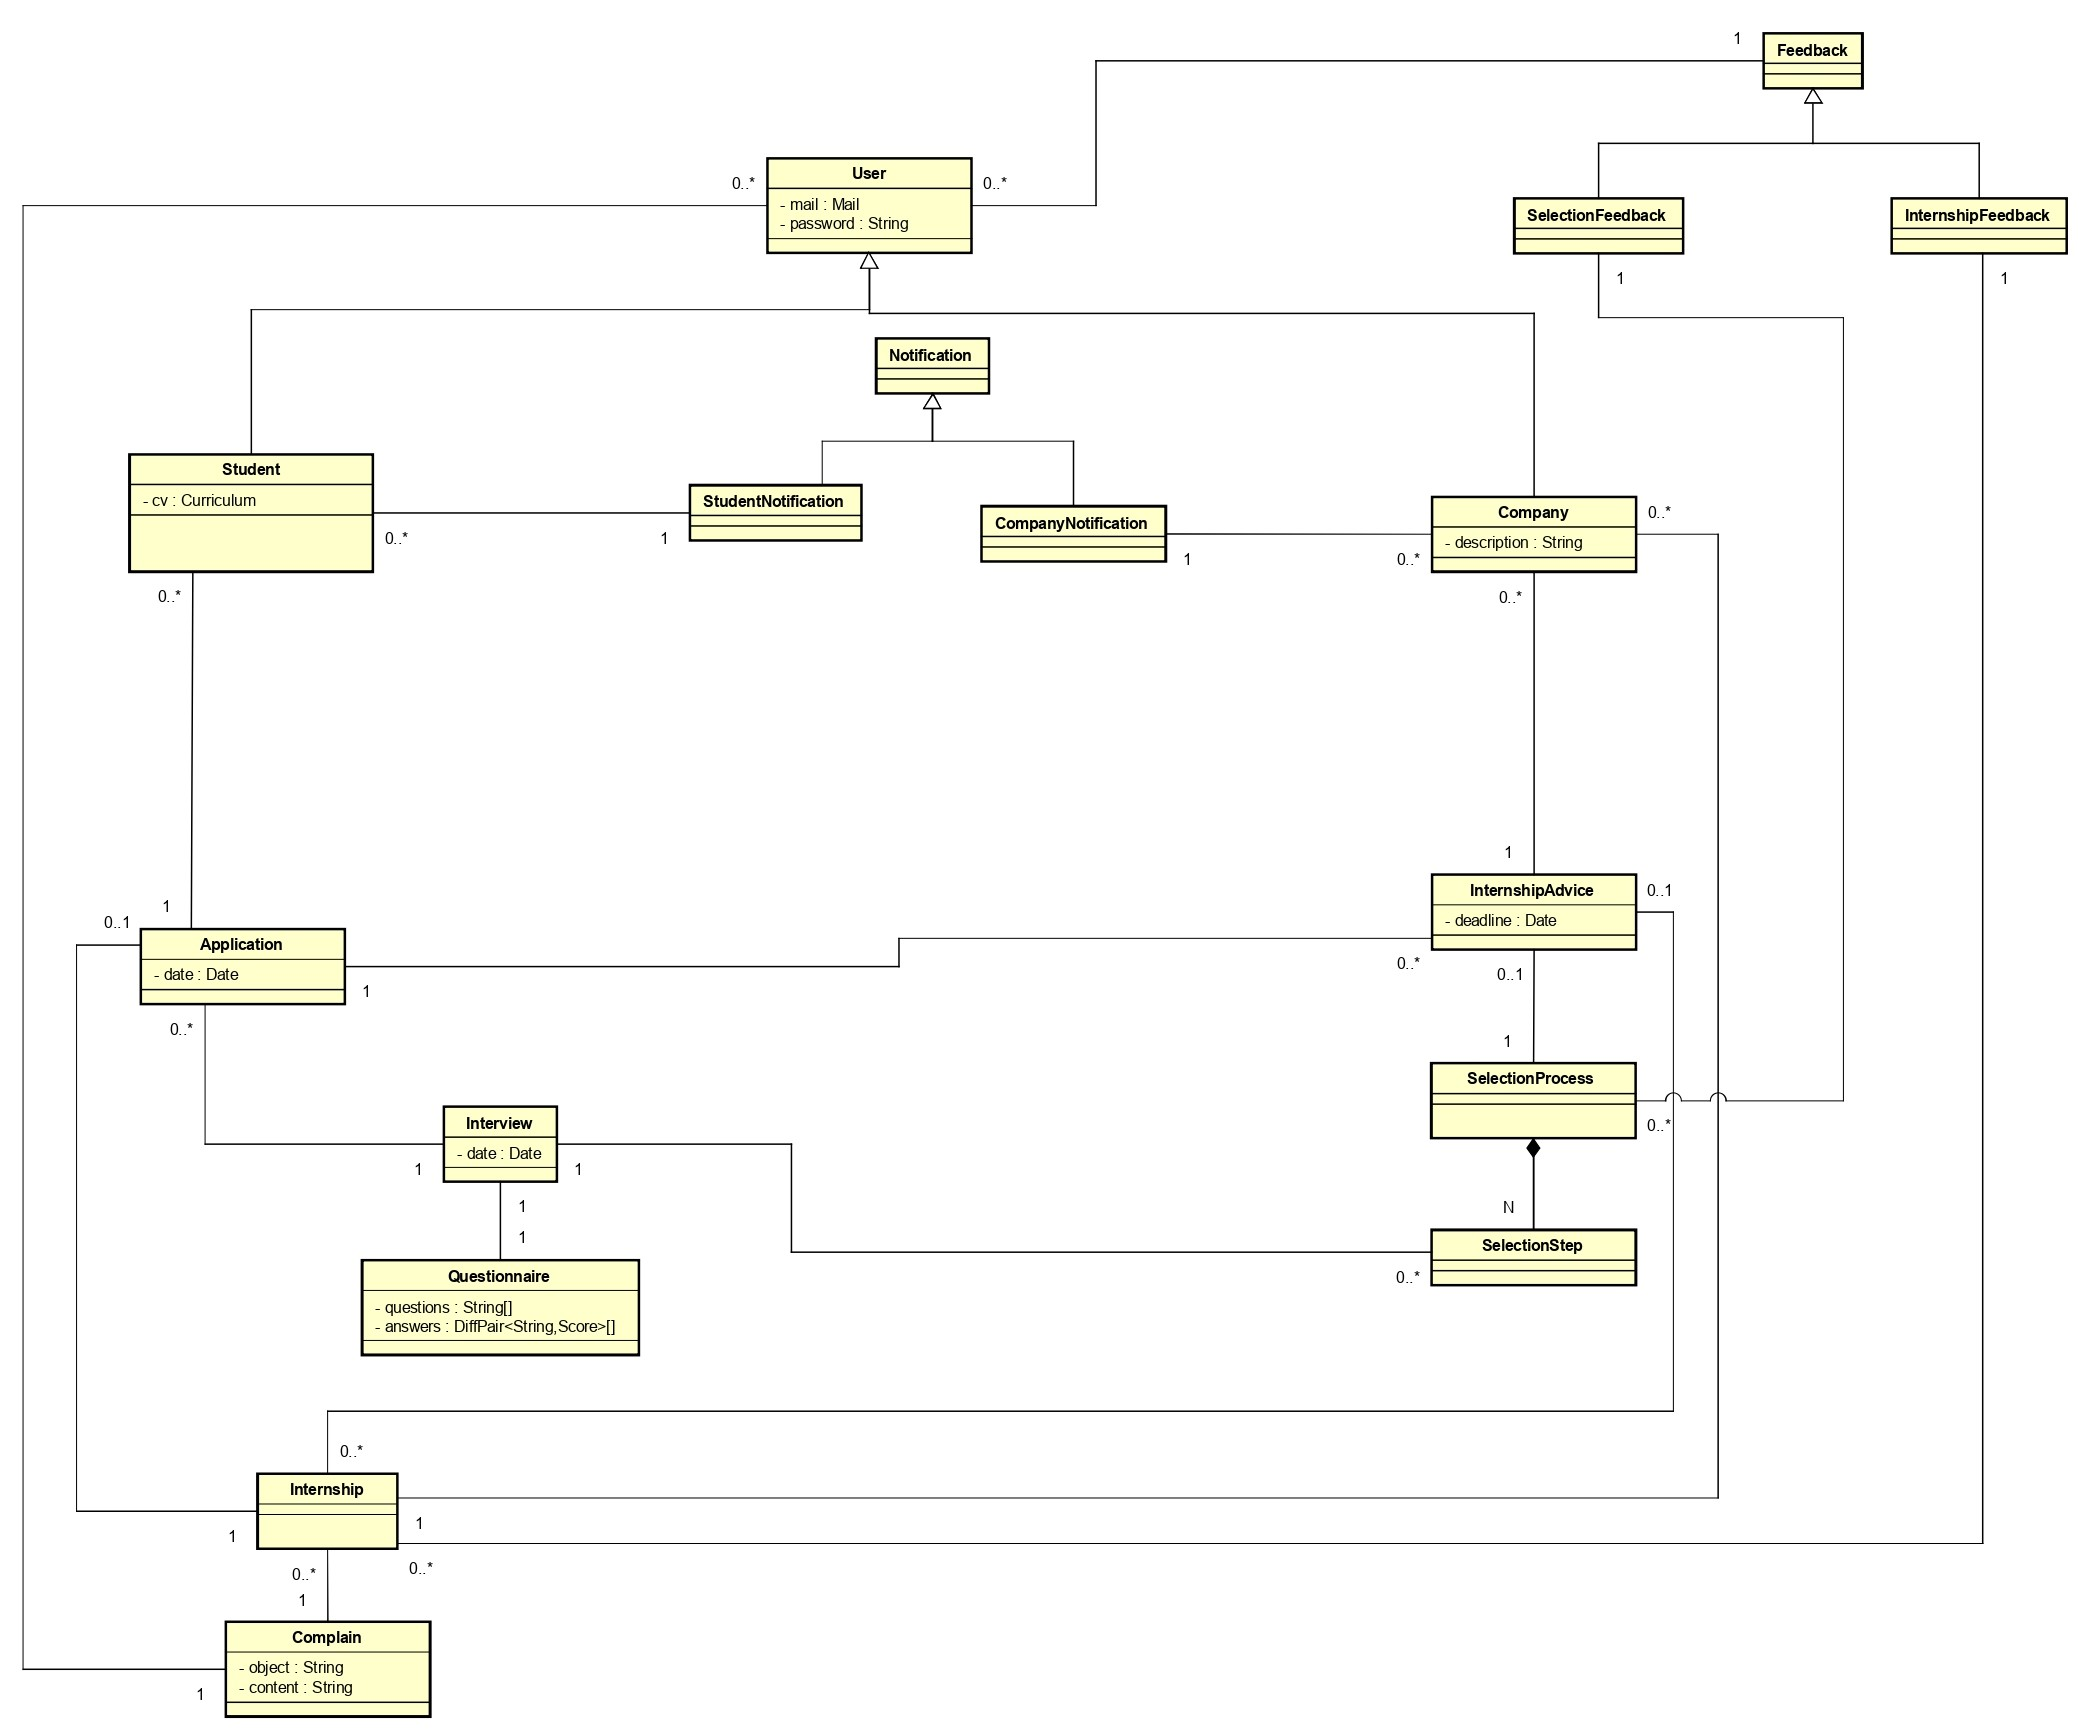
\includegraphics{class_diagram(NO NOT).jpg}
			
			This figure represent the domain class diagram of the system. It represents the fact that the system connects students and companies, facilitating the management of applications, selection processes, interviews, internships, and communication between the parties. It provides tools for sending notifications, collecting feedback, and managing questionnaire and complaints.
			
			The system's users are modeled through the \textit{User} class, which represents both Students (class \textit{Student}) and Companies (class \textit{Company}). Each user has basic attributes (email and password) and can receive personalized notifications (class \textit{Notification}, with subtypes for students and companies).
			
			Companies can publish internships advice (class \textit{InternshipAdvice}), and a student's application for an internship is managed by the \textit{Application} class. Company can also send a proposal of application (class \textit{Proposal)} to a student for one of its internships advice.
			
			Each application can go through a \textit{SelectionProcess}, divided into several \textit{SelectionStep}. During the selection process, the student may undergo an interview (\textit{Interview} class) and his answers are collected by the system through questionnaires (\textit{Questionnaire} class).
			
			Internship advice is associated with a concrete Internsihp (class \textit{Internship}) offered by companies; Internships are linked to feedback (\textit{InternshipFeedback}) and complaints (\textit{Complain}). 
			The system supports the collection of feedback in two forms:
			\begin{itemize}
				\item \textit{SelectionFeedback}: feedback on the selection processes.
				\item {InternshipFeedback}: feedback related to internships
			
			\end{itemize}
			
			
			
			
			
			
			
			
			
			\subsection{State Diagrams}
				In this subsection, the most relevant state diagrams are presented in order to better understand the system's evolution through its different phases. We focus in particular on the representation of an internship's state and the evolution of a student's application.
				
				\subparagraph{State of an internship}
					\begin{center}
						\includegraphics[scale=0.3]{stateInternship.jpg}
					\end{center}
					
					In this state diagram, each state represents the status an internship can have. \textit{Activated} is the state where the internship is published and visible on the platform (in the form of an internship advice); \textit{Under Selection} is the state where the company is conducting the selection process;\textit{Assigned} is the state where the internship has been assigned to specific students; \textit{Closed} is the state where the internship has ended (either because it finished or was interrupted); \textit{Deleted} is the state where the internship is removed from the system (the company deletes the internship advice).
					
				\subparagraph{State of an application for an internship}
					\begin{center}
						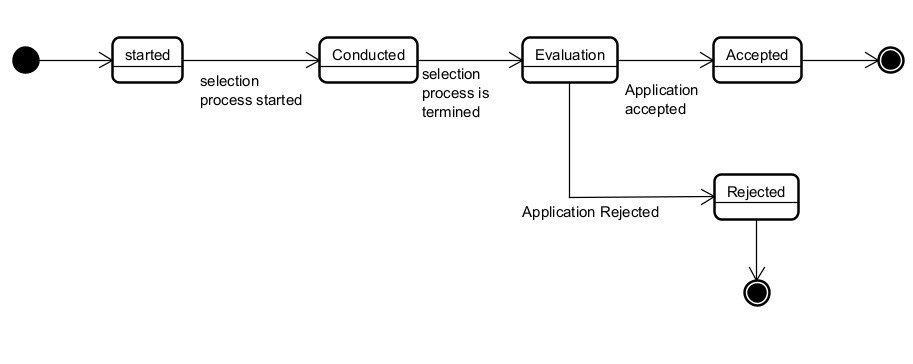
\includegraphics[scale=0.3]{application.jpg}
					\end{center}
					
					In this state diagram, the evolution of a student's application for an internship is described. The \textit{Started} state refers to a student's application for an internship. The \textit{Conducted} state relates to the evolution of the selection process (open questions, closed questions, interviews, questionnaire completion, etc.). The \textit{Evaluation} state is where the company assesses the student's application. From this state, two subsequent states are possible: \textit{Accepted} if the application is accepted, or \textit{Rejected} if it is declined.
					
	\section{Product functions}
		\textbf{Sign-up and login}
			\begin{flushleft}
				This functionality permits to both students and companies to set up their personal profile on the platform and accessing to the latter via their personal information (e-mail and password). Students profiles specify basic information regarding students interests and include their CV while companies profile include all the information that may help student in understanding companies vision and business area.
			\end{flushleft}
		\textbf{Internship proposal management}
			\begin{flushleft}
				Companies can post advice for internship they are going to offer and students can proactively search for them. In this case, a student that wants to apply for an internship sends a request to the company and it decides or not to enroll the student into the selection process. Moreover, thanks to the recommendation feature, companies receives profiles of possibly interested students and students receive profiles of companies that offer internship possibly related to their interests. Therefore, a companies can also suggest to a student to apply for an internship selection and students can accept or decline this proposal.
			\end{flushleft}
		\textbf{Recommendation mechanism}
			\begin{flushleft}
				This functionality aims to facilitate the establishment of a contact between students and companies. By means of recommendation analysis, the system is able to propose to students internships advice that may interest them and to companies students that may be interested to their internships. This analysis are supported by companies and students profiles (CVs in particular, for students) and not compulsory feedback collected at the end of selections processes or internships.
			\end{flushleft}
		\textbf{Selection process management}
			\begin{flushleft}
				A selection process can be supported by the system from the advice deadline to its finalization. In particular, companies can use the system to define process steps, schedule interviews, correct closed questions and compare students results each other (by defining their metrics).
			\end{flushleft}
		\textbf{Internship monitoring}
			\begin{flushleft}
				Students that are currently involved in active internships can use the system to post complains and monitor the current status of them. On the other side, also companies can also post complains on internships they are currently providing (and of course they can also monitor their status).
			\end{flushleft}
		\textbf{Notifications management}
			\begin{flushleft}
				Each message that is sent to companies or students (e.g. selection results, internship proposal, interview dates) are also sent to profile e-mail addresses (a short version of them). From the system, each message can be read entirely.
			\end{flushleft}
	\section{User characteristics}
		there are mainly two types of user that interact with the platform: Student and Companies.
		\subsection{Student}
			The student, once logged into the platform, is able to proactively search for internship advice that may interest them. Once the internship of interest has been selected, they can apply for an interview directly through the platform. Additionally, the student receives a list of possible internships that may suit them, based on their studies/CV, via the aforementioned recommendation mechanism. Furthermore, the student may also receive a proposal to apply directly from the company offering the internship. Once they have completed a selection process, the student will receive the outcome directly through the platform.
		
		\subsection{Comapny}
			The company, once logged into the platform, can publish internship announcements it wants to offer. The system will periodically send the company a list of potential students who may be suitable for their internships, based on their CVs, to whom it can directly send a proposal to apply for one of its internships. Conversely, the company can also accept or reject a student's application. For a given internship, once the application period has ended, the company can schedule the selection process for each candidate directly through the system. During the selection phase, the company also collects all candidate responses using the system.Finally, the company will provide the outcome of the selection to each student directly through the platform.
		
		\subsection{common characteristics}
			Both users can also provide feedback on the selection process as well as at the end of the internship. This feedback is collected by the system to improve the recommendation process. Additionally, both users can monitor the status of an outgoing internship and provide information or complaints about it.
		
	\section{Assumptions, dependencies and constraints}
		\subsection{Domain Assumption}
			the following assumption are made for domain. They are properties or condition that the system will take for granted. They must be checked to ensure a correct platform behaviour.
			
			[D1] Users must have a reliable internet connection
			
			[D2] When users log in, the credentials they enter must be correct
			
			[D3] Informations contained in the CVs are truthful
			
			[D4] Company properly fill the form about internship adivce
			
			[D5] Company correctly enters the answers provided by the student during the interview into the system
			
			[D6] Notifications to users must be delivered as quickly as possible (according with the requirements defined for each notification)
			
		\subsection{Dependencies}
			\begin{itemize}
				\item The system will integrate with email system to send notifications to Users
			\end{itemize}
		
		\subsection{Constraints}
			\begin{itemize}
				\item The system shall be compliant to local laws and regulations, in particular users data should be treated
				according to the GDPR. This means that users should be always able to request their data
				\item The data collected for matching (feedback, ...) are sufficiently detailed to support effective statistical analysis.
				\item The number of students and companies using the platform will be manageable by the system without compromising its performance
				\item To better protect the users’ sensitive information their data should be encrypted (An example is the digital signature on CVs)
			\end{itemize}
		